\section*{Modulazione Numerica in Banda Passante}

\subsection*{Segnale Passa Banda}

Il segnale passa banda può essere espresso come:
\[
s(t) = a(t) \cos[2\pi f_0 t + \phi(t)]
\]
dove \( a(t) \) è l'inviluppo reale di \( s(t) \) (segnale passa-basso) e \( \phi(t) \) la fase di \( s(t) \).



\begin{tikzpicture}[font=\small,>=stealth',thick, node distance=2cm]
\tikzstyle{block} = [rectangle, draw,
    text width=5em, text centered, minimum height=2.5em]
\tikzstyle{signal} = [draw,->]
\tikzstyle{modulator} = [circle, draw, inner sep=0pt, minimum size=1cm]

\node[block] (filter) {p(t)};
\node[modulator, right of=filter, node distance=3cm] (modulator) {\Large$\times$};
\node[above of=filter, node distance=1cm] (input) {x(t)};
\node[right of=modulator, node distance=3cm] (output) {s(t)};

\draw[signal] (input) -- (filter);
\draw[signal] (filter) -- (modulator);
\draw[signal] (modulator) -- (output);
\draw[signal] (filter) -- node[above] {baseband} (modulator);
\draw[signal] (modulator.east) -- node[above] {passband} (output);

\node[above of=modulator, node distance=1cm] (carrier) {cos(2$\pi$f0t)};
\draw[signal] (carrier) -- (modulator);

\end{tikzpicture}


Espandendo l'inviluppo complesso di \( s(t) \), otteniamo:
\[
s(t) = \Re\left\{ a(t) e^{j[2\pi f_0 t + \phi(t)]} \right\}
\]
\[
= \Re\left\{ a(t) \cos[2\pi f_0 t + \phi(t)] + j \cdot a(t) \sin[2\pi f_0 t + \phi(t)] \right\}
\]
\[
= a(t) \cos[2\pi f_0 t + \phi(t)] = \Re\left\{ \tilde{a}(t) e^{j2\pi f_0 t} \right\}
\]
dove \( \tilde{a}(t) \) è l'inviluppo complesso di \( s(t) \).



















\begin{tikzpicture}[>=Stealth, 
    block/.style={draw, rectangle, minimum height=2em, minimum width=3em},
    sum/.style={draw, circle, node distance=1cm},
    node distance=2cm and 3cm
]
    % Nodes
    \node[block] (pfilter) {$p(t)$};
    \node[sum, right of=pfilter] (mixer) {$\times$};
    \node[right= of mixer] (output) {$s(t)$};
    \node[above= of mixer] (cosine) {$\cos(2\pi f_0 t)$};
    \node[left= of pfilter] (input) {$x(t)$};
    
    % Lines
    \draw[->] (input) -- (pfilter);
    \draw[->] (pfilter) -- (mixer);
    \draw[->] (mixer) -- (output);
    \draw[->] (cosine) -- (mixer);

    % Lower part with s tilde
    \node[block, below= of pfilter] (pfilter2) {$p(t)$};
    \node[sum, right of=pfilter2] (mixer2) {$\times$};
    \node[right= of mixer2] (output2) {$\tilde{s}(t)$};
    \node[above= of mixer2] (exponential) {$e^{j2\pi f_0 t}$};
    \node[left= of pfilter2] (input2) {$\tilde{x}(t)$};
    
    % Lines for lower part
    \draw[->] (input2) -- (pfilter2);
    \draw[->] (pfilter2) -- (mixer2);
    \draw[->] (mixer2) -- (output2);
    \draw[->] (exponential) -- (mixer2);
    
    % Draw the constellation diagram
    \begin{scope}[shift={($(output2.south east)+(3cm,-1cm)$)},scale=0.5]
        \draw[->] (-4,0) -- (4,0) node[below] {$\Re$};
        \draw[->] (0,-3) -- (0,3) node[left] {$\Im$};
        
        % Points in the constellation
        \foreach \x in {-3,-1,1,3}
            \fill[orange] (\x,0) circle (5pt);
            
        % Label for n=4
        \node[below] at (3,0) {$n=4$};
    \end{scope}
\end{tikzpicture}








% Definizione di M-PAM
\[
M-PAM \quad \Rightarrow \quad \text{simboli:} \quad A_s = \{\alpha_1, \dots, \alpha_M\}
\]
\[
\alpha = 2c - 1 - M
\]
\[
p(t) = \text{impulso in TX}
\]

% Definizione del segnale s(t)
\[
s(t) = \sum_{n=-\infty}^{\infty} x(n) p(t - nT_s) \cos(2\pi f_c t)
\]

% Diagramma segnale
\begin{tikzpicture}
\node (x) at (0,0) {$x(n)$};
\node[right=2cm of x] (p) {$p(t)$};
\node[right=2cm of p] (s) {$s(t)$};
\draw[->] (x) -- (p);
\draw[->] (p) -- (s) node[midway,above] {$\times$} node[midway,below] {$\cos(2\pi f_c t)$};
\end{tikzpicture}

% Altre espressioni del segnale
\[
\tilde{S}(t) = \sum_{n=-\infty}^{\infty} x(n) p(t - nT_s)
\]
\[
\tilde{s}(t) = \Re\{\tilde{S}(t) e^{j2\pi f_c t}\}
\]
\[
= \Re \left\{ \sum_{n=-\infty}^{\infty} x(n) p(t - nT_s) e^{j2\pi f_c t} \right\}
\]
\[
= \sum_{n=-\infty}^{\infty} x(n) p(t - nT_s) \cos(2\pi f_c t) + j \sin(2\pi f_c t)
\]

% Diagramma dei simboli
\begin{tikzpicture}
\draw[->] (-3.5,0) -- (3.5,0) node[anchor=west] {$\Re$};
\draw[->] (0,-2) -- (0,2) node[anchor=south] {$\Im$};
\foreach \x in {-3,...,3}
  \draw (\x,0.1) -- (\x,-0.1) node[anchor=north] {$\x$};
\foreach \y in {-1,1}
  \draw (0.1,\y) -- (-0.1,\y) node[anchor=east] {$\y$};
% Aggiungere punti qui se necessario
\end{tikzpicture}
\noindent Modulazione di fase PSK (Phase Shift Keying):

% Definizione del segnale s(t)
\begin{flalign}
& s_c(t) = p(t) \cos(2\pi f_0 t + \theta_i) && \text{(simbolo $i$-esimo)} & \\
& \theta_i = \frac{2\pi}{M}(i-1) && \text{per $i = 1, \ldots, M$} &
\end{flalign}

\noindent Espansione del segnale s(t) come sommatoria:

\begin{flalign}
& s(t) = \sum_{n=-\infty}^{\infty} p(t - nT_s) \cos(2\pi f_0 t + \theta_i(n)) & \\
& \theta_i(n) \in A_s = \{\theta_1, \ldots, \theta_M\} &
\end{flalign}

\noindent Definizione del segnale modulato in fase $\tilde{s}_c(t)$:

\begin{flalign}
& \tilde{s}_c(t) = p(t) e^{j\theta_i} & \\
& \tilde{s}_c(t) = \Re\{p(t) e^{j\theta_i} e^{j2\pi f_0 t}\} & \\
& \phantom{\tilde{s}_c(t)} = \Re\{p(t) e^{j(2\pi f_0 t + \theta_i)}\} & \\
& \phantom{\tilde{s}_c(t)} = p(t) \cos(2\pi f_0 t + \theta_i) &
\end{flalign}

\noindent Definizione di $x(n)$ basata su $\theta_n$:

\begin{flalign}
& x(n) = e^{j\theta_n} &
\end{flalign}
% Equations arranged in a row
\noindent
\begin{minipage}{.5\linewidth}
\begin{equation*}
    s(t) = \Re \{ s(t) e^{j 2\pi f_0 t} \}
\end{equation*}
\begin{equation*}
    s(t) \approx \sum_{n=-\infty}^{\infty} s_n e^{j \Omega_n}
\end{equation*}
\end{minipage}%
\begin{minipage}{.5\linewidth}
\begin{equation*}
    s(t) = \Re \left\{ \sum_{n=-\infty}^{\infty} p(t-nT_s) e^{j (2\pi f_0 t + \Omega_n)} \right\}
\end{equation*}
\end{minipage}

% Another row of equations
\noindent
\begin{minipage}{.5\linewidth}
\begin{equation*}
    \approx \sum_{n=-\infty}^{\infty} p(t+nT_s) \cos(2\pi f_0 t + \Theta_n)
\end{equation*}
\end{minipage}%
\begin{minipage}{.5\linewidth}
\begin{equation*}
    S_i(t) = A_{I_i} p(t) \cos(2\pi f_0 t) - A_{Q_i} p(t) \sin(2\pi f_0 t)
\end{equation*}
\end{minipage}

% TikZ Diagram in a row with QAM explanation
\noindent
\begin{minipage}[c]{0.3\linewidth}
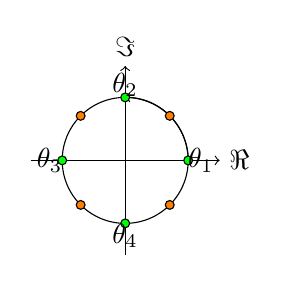
\begin{tikzpicture}[scale=0.8]
    \draw[->] (-1.5,0) -- (1.5,0) node[right] {$\Re$};
    \draw[->] (0,-1.5) -- (0,1.5) node[above] {$\Im$};
    \draw (0,0) circle (1cm);
    \draw[->] (1,0) arc (0:90:1cm);
    \foreach \angle/\label in {0/\theta_1, 90/\theta_2, 180/\theta_3, 270/\theta_4}{
      \draw[fill=green] (\angle:1cm) circle (2pt);
      \node at (\angle:1.2cm) {$\label$};
    }
    \foreach \angle in {45,135,225,315}{
      \draw[fill=orange] (\angle:1cm) circle (2pt);
    }
\end{tikzpicture}
\end{minipage}%
\begin{minipage}[c]{0.7\linewidth}
\begin{equation*}
    \frac{A_{I_i}}{A_{Q_i}} \text{ -- verso e ampiezza della modulazione}
\end{equation*}
\begin{equation*}
    i \text{ -- indice del simbolo } x(t)
\end{equation*}
\end{minipage}




% Start of the content
\[
A^c_i = \text{componente in fase di } x(t)
\]
\[
A^s_i = \text{componente in quadratura di } x(t)
\]

\[
s^c_i(t) = (A^c_i + j A^s_i) p(t)
\]

\[
\Re\{s^c_i(t) e^{j2\pi f_0t}\} = \Re\{(A^c_i + A^s_i) p(t) e^{j2\pi f_0t}\}
\]

\[
= \Re\{A^c_i p(t) e^{j2\pi f_0t} + j A^s_i p(t) e^{j2\pi f_0t}\}
\]

\[
= \Re\{A^c_i p(t) \cos(2\pi f_0t) + j A^c_i p(t) \sin(2\pi f_0t) + A^s_i p(t) \cos(2\pi f_0t) - A^s_i p(t) \sin(2\pi f_0t)\}
\]

\[
= A^c_i p(t) \cos(2\pi f_0t) - A^s_i p(t) \sin(2\pi f_0t)
\]

\[
s(t) = \sum_{n=-\infty}^{+\infty} x_n p(t-nT_s) \cos(2\pi f_0t) - x_s p(t-nT_s) \sin(2\pi f_0t)
\]

\[
s(t) = \Re\{\sum_{n=-\infty}^{+\infty} x_n p(t-nT_s)e^{j2\pi f_0 t}\}
\]

\[
    x[n] = x_c[n] + jx_s[n]
\]

